\section{Простые вычисления}

\textbf{Задание:} Вычислить значение выражения ~$\displaystyle \frac{\cos{x} + \sin{y}}{\ln(x + y)}$
\vspace{0.25cm}

Создано окно, содержащее три элемента TextBox, три элемента Label и 
один элемент Button. Вид окна представлен на рисунке \ref{fig:form2}.

\begin{figure}[H]
    \centering
    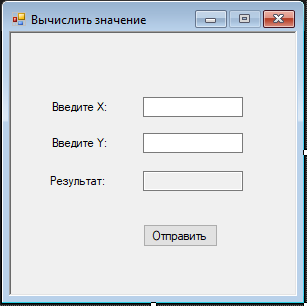
\includegraphics{task2/form.png}
    \caption{Внешний вид формы в конструкторе}
    \label{fig:form2}
\end{figure}

У элементов изменены значения некоторых атрибутов. 
Значения измененных атрибутов представлены в таблице \ref{table:params2}.

\begin{table}[H]
    \small
    \caption{Значения атрибутов элементов в приложении <<Простые вычисления>>}\label{tab:fact-attr}
    \begin{tabular}{|l|l|}\hline
    Наименование атрибута & Значение\cr\hline
    \multicolumn{2}{|l|}{Для формы}\cr\hline
    \verb"Text" & \verb"Вычислить значение"\cr\hline
    \verb"FormBorderStyle" & \verb"FixedSingle"\cr\hline
    \verb"MaximizeBox" & \verb"False"\cr\hline
    \multicolumn{2}{|l|}{Для первой надписи}\cr\hline
    \verb"(Name)" & \verb"xLabel"\cr\hline
    \verb"Text" & \verb"Введите X"\cr\hline
    \multicolumn{2}{|l|}{Для второй надписи}\cr\hline
    \verb"(Name)" & \verb"yLabel"\cr\hline
    \verb"Text" & \verb"Введите Y"\cr\hline
    \multicolumn{2}{|l|}{Для третьей надписи}\cr\hline
    \verb"(Name)" & \verb"lblOutput"\cr\hline
    \verb"Text" & \verb"Результат:"\cr\hline
    \multicolumn{2}{|l|}{Для первого текстового поля}\cr\hline
    \verb"(Name)" & \verb"xInput"\cr\hline
    \multicolumn{2}{|l|}{Для второго текстового поля}\cr\hline
    \verb"(Name)" & \verb"yInput"\cr\hline
    \multicolumn{2}{|l|}{Для третьего текстового поля}\cr\hline
    \verb"(Name)" & \verb"txtOutput"\cr\hline
    \multicolumn{2}{|l|}{Для кнопки}\cr\hline
    \verb"(Name)" & \verb"btnCalculate"\cr\hline
    \verb"Text" & \verb"Вычислить"\cr\hline
    \multicolumn{2}{|l|}{Для обработчика ошибок}\cr\hline
    \verb"(Name)" & \verb"errorProvider1"\cr\hline
    \end{tabular}
    \label{table:params2}
\end{table}

Для работы программы была написана функция вычисления заданного выражения:
\inputminted[fontsize=\small, breaklines=true, style=bw, linenos]{cpp}{task2/f.h}
и функция, проверяющая выбранное поле на корректность:
\begin{minted}[fontsize=\small, breaklines=true, style=bw, linenos]{asm}
    bool VarValidation(System::Windows::Forms::TextBox^ Input, ll& x) { // Проверка числа для поля x из текста объекта Input
		
		ll InputNumber;
		bool IsVariableValid = Int64::TryParse(Input->Text, InputNumber); // Пробуем записать в InputNumber число из потока
		
		if (!IsVariableValid) { // Если не вышло
			errorProvider1->SetError(Input, "Переменная не целое число");
			return 0;
		}
		x = InputNumber; // Обновляем значение переменной
		return 1;
    }
\end{minted}
Логику работы программы реализует фрагмент кода, привязанный к кнопке
\begin{minted}[fontsize=\small, breaklines=true, style=bw, linenos]{cpp}
	private: System::Void btnCalculate_Click(System::Object^ sender, System::EventArgs^ e) {
		ClearAll();

		ll x = 0;
		ll y = 0;

		bool XisOkay = VarValidation(xInput, x); // Проверяем корректность x
		bool YisOkay = VarValidation(yInput, y); // Проверяем корректность y

		if (!XisOkay || !YisOkay) return; // Если какая-то из них некорректна - завершим работу. Все необходимые выводы исключений уже были произведены

		ll summary = x + y; // Считаем сумму для логарифма

		if (summary == 1) { // Если аргумент равен единице - логарифм равен нулю
			errorProvider1->SetError(txtOutput, "Деление на ноль");
			return;
		}

		if (summary <= 0) { // Если аргумент меньше нуля - неверно
			errorProvider1->SetError(txtOutput, "Недопустимое значение для логарифма");
			return;
		}

		double OutputNumber = f(x, y); // Получаем значение функции для заданных чисел х, у

		txtOutput->Text = System::Convert::ToString(OutputNumber); // Отображаем ответ
	}
\end{minted}

Функция \verb|ClearAll()| реализует очищение полей от ошибок.
После запуска приложения на экране появляется окно (см. рисунок \ref{fig:exec2})
\begin{figure}[H]
    \centering
    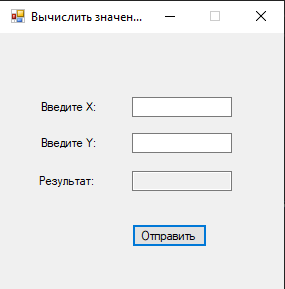
\includegraphics{task2/exec.png}
    \caption{Скриншот запуска программы}
    \label{fig:exec2}
\end{figure}
При вводе целого числа после нажатия кнопки в поле вывода приводится
результат вычисления факториала для заданного числа (см. рисунок \ref{fig:result2}).
\begin{figure}[H]
    \centering
    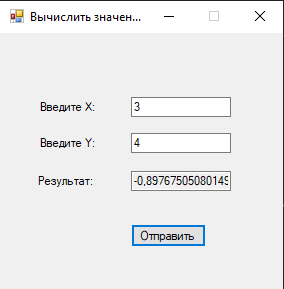
\includegraphics{task2/result.png}
    \caption{Результат работы}
    \label{fig:result2}
\end{figure}
Ввод некорректных значений обрабатывается элементом \verb|errorProvider1| и 
сопровождается сообщением об ошибке (см. рисунок \ref{fig:error2} )
\begin{figure}[H]
    \centering
    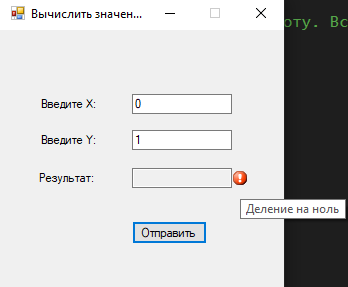
\includegraphics{task2/error.png}
    \caption{Сообщение об ошибке}
    \label{fig:error2}
\end{figure}
Полный код программы приведен в приложении А.